% ---------------------------------------------------------------------------
% §4 RESULTS — paste-ready revize.
% Uygulananlar: config yeniden numaralandırma (eski C7→C6, C11→C10, C3→C2,
% C4→C3, C8→C7, C9→C8, C10→C9); nihai protokoller (binary: C6+direct+T=0;
% Likert: C6+Gemini 2.5 Flash Lite+VS+T=0.8); "protest-positive recall";
% tablo düzenlemeleri (CV sütunu çıktı, T'den sonra dikey çizgi, womenwork
% tablosuna model sütunu + kappa_w); stres testi paragrafına natural-rewrite
% cümlesi; "political-context"→"ideology background"; bazı appendix
% referansları footnote'a.
%
% TODO'lar (yorumlarda işaretli):
%  (1) figures/final_picks_vs_gt.png YENİDEN üretilmeli: yeni protokoller
%      C6+direct+T0 (pacdemons) ve C6+Gemini+VS+T0.8 (womenwork) ile
%      (script: scripts/plot_final_picks_vs_gt.py).
%  (2) pacdemons T=0 hücresinin simulated positive rate'i figür koşusundan
%      alınıp metne eklenecek.
%  (3) Appendix F (app:stability) yeni protokollerin çok-tohumlu koşularıyla
%      güncellenmeli; eski "Gemini istikrarsız" cümlesi kaldırılmalı.
%  (4) §3 dosyasındaki \ref{sec:results} → \ref{sec:calibration-results}.
% ---------------------------------------------------------------------------

\section{Results}
\label{sec:calibration-results}

\subsection{Calibration Results}

This section reports the empirical record produced by the calibration
funnel. Four results organize the analysis. First, calibration performance
is outcome-specific: the same inference setup does not perform best across
the rare binary participation item and the ordered Likert attitude item.
Second, among the components we vary, the choice of what respondent
information enters the persona changes performance most; sampling strategy
matters next, and model family, temperature, and prompt presentation
produce comparatively minor differences. Third, distributional and
respondent-level recovery must be carried together, because a setup that
excels on one can quietly fail the other: a protocol can reproduce the
marginal distribution almost exactly while identifying almost none of the
true affirmative cases, and one that tracks an ordered distribution closely
can retain little respondent-conditional signal. Fourth, and most
consequentially for practice, these results are properties of the pairing
between a model and a target rather than of the model alone. An
experimental design of this kind should therefore be preceded by a
calibration stage evaluated against ground truth substantively related to
the experiment, with the selected combination frozen before any treatment
response is generated. We follow that sequence here, selecting separate
final protocols for the two outcomes before the synthetic population enters
the downstream experiment.\footnote{Full cell-level results and
implementation details are reported in
Appendix~\ref{app:calibration-results}.}

The largest performance differences come from persona content. Varying the
persona configuration while holding the inference setup fixed at direct
answering, temperature zero, first-person address, and GPT-4o-mini already
separates the candidate setups more sharply than any later step in the
funnel. For
\textit{pacdemons}, protest-positive recall ranges from near zero under the
demographic-only baseline (0.01, C0) to roughly half of true participants
(0.51, C6 and C8), even though Jensen--Shannon divergence remains below
0.02 across configurations.\footnote{C0 retains only the respondent's basic
demographic block. Its near-complete failure to detect affirmative
responses motivates the inclusion of socioeconomic, political, and
attitudinal information in richer configurations.} This contrast shows why
rare protest participation cannot be evaluated with distributional fit
alone: a model can match the marginal distribution while failing to
identify almost all true affirmative cases. The failure of C7 and C9
reinforces this point: both configurations collapse on \textit{pacdemons}
after politically relevant information blocks are removed
(protest-positive recall below 0.10).

Persona content matters just as much for \textit{womenwork}. Across the
screening stage Wasserstein distance nearly halves, from 0.94 under the
demographic-only baseline to 0.49 under the best-performing profile --- a
spread as consequential on the ordered scale as the recall spread is on the
binary one. What the two outcomes do not share is a single ranking of
profiles. Richer political and socioeconomic information helps
\textit{pacdemons} recover rare affirmative responses, whereas at this
stage the leaner C10 profile attains the closest distributional fit for
\textit{womenwork}. That ordering should be read as provisional: it is
measured under one sampling strategy, one model, and a purely
distributional criterion, and it does not survive once those components are
varied and respondent-level agreement is brought into the comparison. What
does hold across both outcomes is that the fullest profile is not
automatically the most accurate. C1 attains the lowest JSD for
\textit{pacdemons} yet misses roughly six in ten true affirmatives, and on
\textit{womenwork} it trails the leading profiles by a wide margin (0.78
against 0.49).

Sampling strategy is the next most consequential choice, and it too depends
on the structure of the outcome. Direct answering outperforms verbalized
sampling for the binary
participation item at every temperature: verbalized sampling raises JSD by
an order of magnitude and weakens respondent-level discrimination across
the shortlisted configurations. For the Likert item, the pattern reverses.
Moving from direct answering to verbalized sampling sharply reduces
Wasserstein distance for the leading configurations (for C10 at $T=0.8$,
from 0.472 to 0.151). Probabilistic answering therefore improves recovery
of a graded attitudinal distribution, while direct answering better
preserves classification performance for the rare affirmative category.

After persona content and sampling strategy are fixed, temperature produces
only modest changes. For \textit{pacdemons} under C6 direct answering,
protest-positive recall moves from 0.51 at $T=0$ to 0.54 at $T=0.8$ with
JSD effectively unchanged; for \textit{womenwork} under verbalized
sampling, Wasserstein distance is flat across temperatures. We therefore
fix $T=0$ for the binary protocol, which keeps the per-respondent
prediction fully deterministic and reproducible, and $T=0.8$ for the Likert
protocol, where the verbalized distribution benefits from a mildly diffuse
generation. This choice should be read as an empirical result for these
outcomes and models rather than as a general recommendation.

Cross-model checks differentiate the two outcomes. For \textit{pacdemons},
GPT-4o-mini is clearly strongest: under C6 direct answering it reaches
protest-positive recall of 0.51--0.54 across temperatures, against 0.44
for GPT-5.4-mini, 0.31 for Llama 3.3 70B, and a collapse to 0.01 for
Gemini 2.5 Flash Lite. For \textit{womenwork}, the comparison depends on
what is being optimized. Under the compact C10 profile, GPT-4o-mini attains
the best distributional fit (Wasserstein 0.151), but its respondent-level
ordinal agreement is weak (quadratic weighted kappa 0.08). Under C6, the
configuration selected for the binary outcome, Gemini 2.5 Flash Lite
attains a Wasserstein distance of 0.218 together with quadratic weighted
kappa of 0.401, roughly five times the ordinal agreement of the
distribution-only leader at a modestly higher Wasserstein distance.

Presentation stress tests produce smaller changes than persona content or
sampling strategy. Switching from first-person to second-person address
moves \textit{pacdemons} protest-positive recall from 0.54 to 0.49 with
JSD unchanged. Adding an explicit reasoning instruction reduces recall to
0.37 while improving marginal fit, again showing why JSD cannot be the only
decision criterion for rare binary outcomes. The ideology background
paragraph leaves both metrics within 0.001 of baseline. For
\textit{womenwork}, second-person address and explicit reasoning leave
Wasserstein distance essentially unchanged. We therefore retain the
baseline presentation in the final protocols. The natural-language rewrite
is the exception that clarifies the rule: presentation choices that leave
the structured variable map intact barely move the results, whereas
dissolving that map into prose halves respondent-level
agreement.\footnote{The rewriting procedure and full results are reported
in Appendix~\ref{app:natural}.}

Before fixing the final protocols, we compare the strongest candidate
setups for each outcome. For \textit{pacdemons}, the shortlist is
restricted to direct answering because verbalized sampling weakens overall
classification performance on the rare binary outcome. For
\textit{womenwork}, the shortlist is restricted to verbalized sampling
because direct answering produces substantially worse Wasserstein distance
on the ordered outcome; candidates are compared jointly on distributional
fit and respondent-level ordinal agreement.
Tables~\ref{tab:final-shortlist-pacdemons}
and~\ref{tab:final-shortlist-womenwork} report the shortlisted candidates.

\begin{table}[H]
\centering
\caption{Final shortlist for \textit{pacdemons} (direct answering,
GPT-4o-mini, first-person address). The primary selection criterion is
respondent-level classification performance under a deterministic protocol.
$\kappa$ = Cohen's kappa; Rec(+) = protest-positive recall (recall on the
rare affirmative class).}
\label{tab:final-shortlist-pacdemons}
\small
\begin{tabular}{@{}clr|rrr@{}}
\toprule
Rank & Config & $T$ & MCC & $\kappa$ & Rec(+) \\
\midrule
1 & C6 & 0.8 & 0.430 & 0.424 & 0.536 \\
2 & C6 & 0.4 & 0.421 & 0.416 & 0.524 \\
3 & C1 & 0.8 & 0.412 & 0.412 & 0.440 \\
4 & C6 & 0.0 & 0.410 & 0.405 & 0.512 \\
5 & C2 & 0.0 & 0.407 & 0.407 & 0.452 \\
\bottomrule
\end{tabular}
\end{table}

\begin{table}[H]
\centering
\caption{Final shortlist for \textit{womenwork} (verbalized sampling,
first-person address). Candidates are evaluated jointly on aggregate
ordinal fit (Wasserstein distance) and respondent-level ordinal agreement
(quadratic weighted kappa, $\kappa_w$).}
\label{tab:final-shortlist-womenwork}
\small
\begin{tabular}{@{}cllr|rr@{}}
\toprule
Rank & Config & Model & $T$ & Wass & $\kappa_w$ \\
\midrule
1 & C6 & Gemini 2.5 Flash Lite & 0.8 & 0.218 & 0.401 \\
2 & C10 & GPT-4o-mini           & 0.8 & 0.151 & 0.082 \\
3 & C10 & GPT-4o-mini           & 0.4 & 0.152 & 0.081 \\
4 & C6 & GPT-5.4-mini          & 0.8 & 0.377 & 0.427 \\
5 & C3 & GPT-4o-mini           & 0.4 & 0.279 & 0.163 \\
\bottomrule
\end{tabular}
\end{table}

The shortlist comparison confirms the outcome-specific selection, and it
converges on a single persona configuration. For \textit{pacdemons}, C6
dominates the shortlist; differences across its temperature variants are
small relative to seed-level variation, so we adopt the deterministic
$T=0$ cell, which recovers roughly half of true protest participants
(protest-positive recall 0.512) at essentially perfect marginal fit. For
\textit{womenwork}, the C10 cells lead on distributional fit alone, but
their respondent-level ordinal agreement is close to chance. C6 on
Gemini 2.5 Flash Lite offers the strongest joint performance: it accepts a
0.07 increase in Wasserstein distance in exchange for roughly five times
the ordinal agreement, and it holds the persona configuration fixed across
the two outcomes. GPT-5.4-mini reaches a similar $\kappa_w$ but at a much
worse distributional fit.

We therefore fix a single persona configuration, C6, for both outcomes,
and let the inference protocol adapt to the response format: direct
answering at $T=0$ on GPT-4o-mini for the rare binary outcome, and
verbalized sampling at $T=0.8$ on Gemini 2.5 Flash Lite for the ordered
Likert outcome. These choices reflect different calibration targets. The
\textit{pacdemons} protocol prioritizes respondent-level discrimination
because the main risk is majority-class collapse. The \textit{womenwork}
protocol balances ordinal distributional alignment, which the downstream
experiment compares across treatment conditions, against respondent-level
ordinal agreement, which anchors the simulated distribution in
respondent-conditional signal. Fixing one persona configuration across
outcomes also simplifies the experimental stage, where both outcome
formats are administered to the same synthetic population.
% TODO (3): Appendix F bu iki protokolün çok-tohumlu koşularıyla
% güncellenmeli; eski metindeki Gemini istikrarsızlık cümlesi kaldırılmalı.

Recall on the rare affirmative class deserves emphasis rather than
apology: the characteristic failure mode of persona-conditioned models on
rare political behavior is to collapse onto the majority class and find
almost no true participants at all, as the demographic-only baseline does
(recall 0.01). The calibrated protocol instead identifies roughly half of
the respondents who actually attended a protest while keeping the
simulated participation rate within two percentage points of the observed
five percent: it gains recall without paying for it in precision.

The distinction between distributional alignment and respondent-level
agreement remains visible in the final diagnostics. For
\textit{pacdemons}, where direct answering produces a deterministic
prediction per respondent, the selected setup reaches MCC 0.410 and
Cohen's kappa 0.405. For \textit{womenwork}, where verbalized sampling
draws responses from a model-stated probability distribution, quadratic
weighted kappa of 0.401 indicates meaningful ordinal agreement, though it
should not be read as strong individual-level prediction; the protocol is
validated as a distributional simulation procedure whose draws retain
respondent-conditional signal.\footnote{Appendix~\ref{app:subgroup}
reports subgroup and regional validation diagnostics for the final
protocols. These diagnostics show that calibration performance is broadly
preserved across major demographic, political, and geographic
subpopulations, with bounded deviations rather than subgroup-level
collapse.}

Figure~\ref{fig:final-picks-vs-gt} provides a direct visual comparison
between the observed TGSS distributions and the simulated distributions
generated by the final calibrated protocols. For \textit{pacdemons}, the
selected C6 direct-answering setup preserves the rarity of the affirmative
category while recovering 51.2\% of true affirmative cases, and the
confusion matrix shows that the protocol does not simply reproduce the
majority class. For \textit{womenwork}, the selected C6
verbalized-sampling setup tracks the observed ordinal distribution, with a
Wasserstein distance of 0.218 and closely matching observed and simulated
means (3.24 and 3.09).
% TODO (1)-(2): figürü yeni protokollerle yeniden üret ve pacdemons T=0
% simulated positive rate'ini buraya ekle.

\begin{figure}[H]
\centering
\includegraphics[width=\textwidth]{figures/final_picks_vs_gt.png}
\caption{Final protocol distributions compared with TGSS ground truth.
Panel (a) compares the observed and simulated response distributions for
\textit{pacdemons} under the final C6 direct-answering protocol at $T=0$
on GPT-4o-mini. The positive class is coded as 1 and denotes participation
in a protest or demonstration in the last 12 months. The confusion matrix
reports respondent-level classification counts for this binary item. Panel
(b) compares the observed and simulated response distributions for
\textit{womenwork} under the final C6 verbalized-sampling protocol at
$T=0.8$ on Gemini 2.5 Flash Lite. The \textit{womenwork} item is coded
from 1 (strongly disagree) to 5 (strongly agree). The empirical CDF panel
visualizes the ordinal distributional fit summarized by Wasserstein
distance. Quadratic weighted kappa is reported as a diagnostic and should
not be interpreted as strong respondent-level prediction accuracy.}
\label{fig:final-picks-vs-gt}
\end{figure}

\subsection{Experimental Results}
\label{sec:exp-results}

This section reports the results of the political-structure experiment. All
estimates are within-persona paired contrasts between the threat (security)
and opportunity (peace) conditions over the full synthetic population.
Subgroup analyses use four respondent characteristics: age, education,
ethnic origin, and left--right self-placement. Respondents whose
characteristic is not reported are excluded from the corresponding
breakdown.

\textbf{Political structure moves both outcomes in the same direction.}
Moving the same protest event from an opportunity to a threat environment
lowers perceived movement legitimacy from 2.34 to 1.98 on the five-point
scale, a within-persona shift of $-0.35$ ($t = -12.1$, $p < .001$,
$d_z = -0.24$), and reduces the share of twins who would attend the march
from 22.8 to 6.7 percent, a shift of $-16.1$ percentage points
($t = -22.4$, $p < .001$, $d_z = -0.44$). The costly behavioral disposition
contracts proportionally far more than the evaluative judgment: the security
environment cuts expressed willingness to attend to less than a third of its
opportunity-condition level, while legitimacy declines but does not
collapse. Figure~\ref{fig:exp-main} summarizes the two contrasts.

\begin{figure}[t]
  \centering
  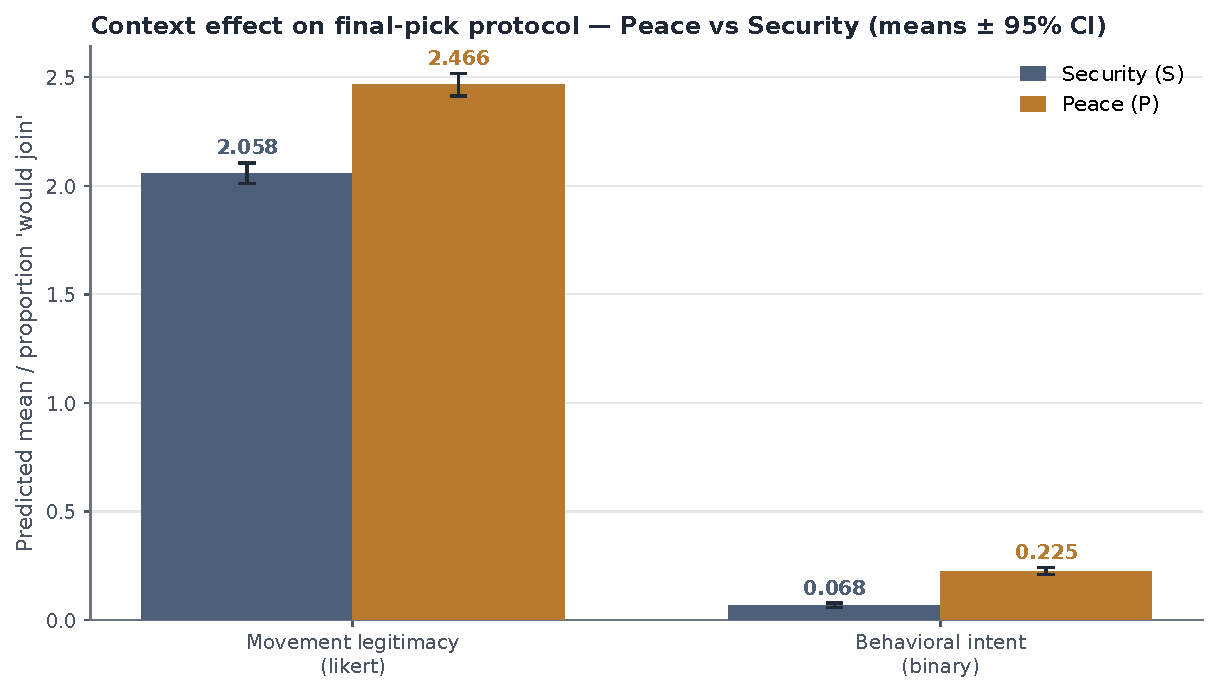
\includegraphics[width=.85\textwidth]{figures/fig_context_main.pdf}
  \caption{Political-structure effect on both outcomes. Points are condition
  means over the full synthetic population ($n = 2{,}615$) with 95\%
  confidence intervals; $p$-values are from within-persona paired
  $t$-tests.}
  \label{fig:exp-main}
\end{figure}

\textbf{Within each political structure, responses are stratified by
politics, ethnicity, and education.} In the opportunity condition, left-placed
twins rate legitimacy 0.47 points above the rest of the population and 55.8
percent of them would attend, against 13.9 percent among the remainder
($d = 0.98$). Kurdish twins rate legitimacy 0.19 points higher than
non-Kurdish twins ($p = .001$) and are substantially more willing to attend
(34.2 versus 19.6 percent, $d = 0.33$). Willingness to attend also rises
monotonically with education and is highest among twins aged 18--29. The
same ordering holds in the threat condition at uniformly lower levels: left
placement ($+0.60$ on legitimacy, $d = 0.53$) and Kurdish origin ($+0.25$,
$d = 0.22$) remain the strongest cleavages, and every one-way test across
the four breakdowns is significant except age on legitimacy.
Figures~\ref{fig:exp-peace-sub} and~\ref{fig:exp-security-sub} report the
subgroup means with the associated tests.

\begin{figure}[t]
  \centering
  \includegraphics[width=\textwidth]{figures/fig_peace_subgroup_signif.pdf}
  \caption{Opportunity (peace) condition: subgroup means and 95\% confidence
  intervals for both outcomes across the four breakdowns. Panel headers
  report the one-way test across subgroup levels (Welch $t$ for two-level
  breakdowns, $F$ otherwise); stars mark the one-vs-rest contrast for the
  focal categories (Kurdish; Left). Respondents with unreported
  characteristics are excluded.}
  \label{fig:exp-peace-sub}
\end{figure}

\begin{figure}[t]
  \centering
  \includegraphics[width=\textwidth]{figures/fig_security_subgroup_signif.pdf}
  \caption{Threat (security) condition: subgroup means, confidence
  intervals, and significance tests, as in
  Figure~\ref{fig:exp-peace-sub}.}
  \label{fig:exp-security-sub}
\end{figure}

\textbf{The size of the political-structure effect is itself politically
structured.} On legitimacy, the largest within-persona shift occurs at the
political center ($-0.44$), with smaller shifts on the left ($-0.26$) and
right ($-0.33$): the ideological poles hold relatively stable evaluations
across environments, while the center moves. On behavioral intent the
pattern reverses in a substantively informative way: the left shifts most
($-35.1$ points), the center shifts moderately ($-17.2$), and the right
barely moves ($-4.1$) because its willingness to attend is near the floor in
both conditions. Kurdish twins likewise shift more than non-Kurdish twins on
intent ($-22.9$ versus $-14.2$ points): the constituencies most willing to
mobilize under the opportunity structure are the ones with the most
mobilization to lose under threat. The full set of subgroup contrasts is
shown in Figure~\ref{fig:exp-forest}.

\begin{figure}[t]
  \centering
  \includegraphics[width=\textwidth]{figures/fig_context_effect_forest.pdf}
  \caption{Within-persona political-structure effect (threat minus
  opportunity) by subgroup, for both outcomes, in a single display. Squares
  are subgroup means of the paired difference with 95\% confidence
  intervals; the dashed line marks the population-level effect. Dark markers
  are significant at $p < .05$.}
  \label{fig:exp-forest}
\end{figure}

\textbf{Evaluations and dispositions respond to the environment, not only to
who is answering.} Because every twin answers under both political
structures, the estimates above cannot be produced by compositional
differences between conditions. The experiment therefore recovers, inside a
calibrated synthetic population, the conditional claim that motivated the
design: the same protest event, advanced by the same movement with the same
claim, elicits systematically weaker public legitimacy and sharply weaker
mobilization potential when it unfolds under threat rather than opportunity,
and the cost of the threat environment falls disproportionately on the
movement's most mobilizable publics.
